\chapter{Algorithm}
\label{chapter:algorithm}

After meticulous research on behaviour and abilities of \textit{Physarum Polycephalum} and acquaintance of Quadratic Assignment Problem field knowledge, we could proceed with design of the new algorithm. Initial concept assumed creating a Physarum Machine --- a method of computation made directly on the slime mould, where inputs are defined by positions of food sources and physical constrains and results can be read via interpretation of slime mould's movements and other behaviours.

Such machine requires specific placement of food sources and constraints which must be transformed from QAP input into positions on physical Petri dish surface. Initial positions of \textit{Physarum} colonies must be declared too. When environment for the experiment is created, scrupulous observations of foraging plasmodium must be continously made --- one can use human observer or automate this process using a camera and image processing software. During the experiment input can be modified if the algorithm requires such step. In the end solution for the QAP can be distilled from the observations. General schematic for universal physarum machine is given on figure \ref{figure:a_machine}.

\begin{figure}
  \centering
  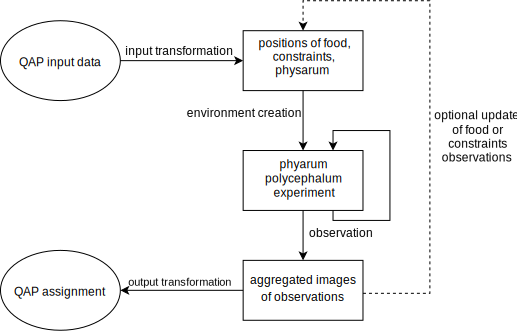
\includegraphics[width=0.84\textwidth]{algorithm/physarum_machine.png}
  \caption{Generic physarum machine schematic}
  \label{figure:a_machine}
\end{figure}

It can be seen that design of the Physarum Machine is a complex task --- methods of communication, observation, food placement, limits formation must be created, not to mention essential two non-trival transformations must be engineered. Quadratic Assignment Problem is defined by two input matrices --- weight matrix and distance matrix. While it is natural to interpret weight matrix as graph of facilities connected with trade relation, one cannot think the same about the location matrix since it depends on the assignment: one of interpretions of the problem is to assign these facilities so transport cost of goods between different facilities is the lowest. Finding the optimal assignment is a complex task, in fact there are $n!$ possible assignments. As previously shown slime moulds have been used to approximate solutions of some graph problems (such as shortest path or networking problem), there are even some approaches to solving Travelling Salesman Problem --- all of these issues have one thing in common, stating the problem in \textit{Physarum} domain, as set of food locations and constraints is trivial as \textit{input transformation} is relatively easy function. 

An obvious challenge is to model QAP input using a \textit{input transformation function}, only when such function is defined, the other part of the machine, \textit{output transformation function} can be designed. The \textit{output transformation} could use movement of plasmodium, oscillations of pseudopodia or other observations to obtain the solution, the final assignment.

Initially we thought of treating the slime mould as restricted linear programming solver, stating the QAP in one of the forms of linearized mathematical programming problems. Literature gives many different approaches for such linearization, but even these did not inspire us for any practical representation in a "slime mould world". Another approach has been proposed, which explores space of all possible assignments using crawling plasmodium. It could have been implemented as physical physarum machine, however it have no practical benefits, requiring lots of preparation and observation overhead. Details of this algorithm are presented it the next section. While it may not be practical, it showed us that we are not capable of designing a better physarum machine, however we took an inspiration from this experience and designed a metaheuristic based on observed behaviour of \textit{Physarum Polycephalum}.

\section{Naive Space Search using Physarum Polycephalum}
\label{section:algorithm_naive}

Using classic definition of Quadratic Assignment Problem, we can assign a cost $c : f \rightarrow \mathbb{R}$, $c(f) = \sum_{a,b\in P}w(a,b)\cdot d(f(a), f(b))$ for each assignment $f$. The goal is to find assignment minizing the cost. To approximate the solution, we propose variation of brute force algorithm implemented as a Physarum Machine.

The input transformation is rather simple: for each possible $n!$ assignments we compute its cost and transform it to size of food source using examplar function $g(c(f)) = \frac{a}{q^{c(f)+k}}+b$, where $a$ and $k$ are scaling factors and $b$ is bias, the exponential function of base $q$ is used to amplify small costs. The parameters of function $g$ can be selected in such manner that small difference in cost is represented by not-so-small difference in food source mass. Food sources of weight $g(c(f))$ made of porridge (sterile oatmeal paste) are placed uniformly on the substrate --- for each assignment there is a respective food source with its size exponentially inversely proportional to the cost. Number of the slime mould colonies in plasmodial stage are placed on this prepared environment. Now observations could be made --- the experiment proceeds as long as plasmodium actively moves within given observation timeframe. 

Exploiting the fact that \textit{Physarum Polycephalum} prefers to consume the biggest food source, an output transformation simply takes position of the plasmodium and returns an assignment linked with physical food source where the plasmodium resides. It should be remembered that the slime mould is a living creature and results obtained using this algorithm are just an approximation as plasmodium behaves nondeterministically when foraging.

Presented algorithm is just a concept and has not been tested in a wet lab as it is highly unpractical. The input transformation requires computing food size for every possible $n!$ assignment, then a human or CNC must place this food on a substrate (which itself must be big enough to contain everything), then long, many days observations must be done until the plasmodium stops crawling. With that much work, we would get only an approximation --- the approximation of $argmin$ function which could have been worked out using a computer giving accurate results, probably in time shorter than time needed for computing the input transformation. 

% TODO dumped idea of physarum machine as highly impractical
% TODO no added quality - it is still n! with longer computing time


\section{Physarum-based Metaheuristic}
\label{section:algorithm_metaheuristic}

Emboldened by the experience with the physarum machine, we thought of making it more practical. We thought of simulating \textit{Physarum Polycephalum}, hoping for lowering execution time for the naive algorithm. Instead we propose a new algorithm designed from the ground up, which is inspired by observed behaviour of the slime mould. While the algorithm was created for solving Quadratic Assignment Problem, it is an universal metaheuristic which can be applied to number of optimization problems.


\subsection{Algorithm overview}

The algorithm can be divided in three distinct phases: exploration, crawling and merging. These phases are executed sequentially in a loop, until stop condition is satisfied. General overview of the algorithm can be seen in pseudocode \ref{algorithm:m_general}. 

\begin{algorithm}[H]
  \KwData{optimization problem with neighbourhood definition}
  \KwResult{approximated result}
  \BlankLine

  environment $\leftarrow$ initialize\_environment(problem)\;
  colony $\leftarrow$ initialize\_colony(environment)\;

  \Repeat{$colony.stable \lor {\neg}experiment.next$}{
    \For{$plasmodium \in colony$}{
      plasmodium.explore()\;
      plasmodium.crawl()\;
    }
    colony.merge()\;
  }

  \Return{colony.largest}\;

  \caption{Overview of physarum-based metaheuristic}
  \label{algorithm:m_general}
\end{algorithm}

Initialization of environment includes sampling of solutions space: $k$ random assignments are taken, for each of them a cost is computed (pseudocode \ref{algorithm:m_env_initialization}). An assignment with the smallest cost is saved as exemplar for further calibration. Colony of "virtual physarum" is put on best $l$ out $k$ samples (pseudocode \ref{algorithm:m_colony_initialization}).

\begin{algorithm}
  \KwData{optimization problem}
  \KwResult{list of samples}
  \BlankLine

  solutions $\leftarrow$ \{\}\;
  \For{$i \leftarrow 0$ \KwTo $k$}{
    solutions $\leftarrow$ solutions $\cup$ \{random\_solution()\}\;
  }

  sorted\_solutions $\leftarrow$ sort(solutions, problem.cost)\;
  environment.best\_cost $\leftarrow$ problem.cost(sorted\_solutions.first)\;
  
  \Return{sorted\_solutions}\;

  \caption{Initialization of environment}
  \label{algorithm:m_env_initialization}
\end{algorithm}

\begin{algorithm}
  \KwData{environment with sampled solutions}
  \KwResult{set of virtual physarum}
  \BlankLine

  colony $\leftarrow$ \{\}\;
  \For{$i \leftarrow 0$ \KwTo $l$}{
    plasmodium $\leftarrow$ create\_plasmodium(environment.samples[i])\;
    colony $\leftarrow$ colony $\cup$ \{plasmodium\}\;
  }
  \Return{colony}\;

  \caption{Initialization of colony}
  \label{algorithm:m_colony_initialization}
\end{algorithm}

Simulation stops when plasmodia crawl no more (are in a stable state) or given number of iterations or time has been exceeded. Result of optimization can be obtained as the solution with the smallest cost which is occupied by a virtual physarum at the end of simulation.


\subsection{Environment}

The naive algorithm assumed uniform distribution of food sources which are inversely proportional to the cost of solution, however there is no such need in our metaheuristic solution. In similar manner solutions are represented as vierual food sources, but they are generated dynamically --- virtual food consume no memory unless they are visited by plasmodium. "Nutritional energy" is calculated dynamically when a food is visited as follows: 

% TODO maybe just frac squared???
\begin{equation}
  E_{solution} = a \cdot q^{\frac{calibrated\_cost}{cost(solution)}} + {\Delta}E_{solution}
\end{equation}

Where $calibrated_cost$ is cost of minimal solution obtained via initial sampling process, $a > 0$ is scaling factor, $q > 1$ is exponentiation base. ${\Delta}E_{solution}$ is already consumed energy from given $solution$. At the start each ${\Delta}E_{solution}$ is equal $0$, so there is no need of storing such information, but as plasmodium explores and crawls ${\Delta}E_{solution}$ is updated, taking at most $O(n!)$ memory if every solution would be explored.

The algorithm defines neighbourhood for Quadratic Assignment Problem as single pair swap, giving $\frac{n\cdot(n-1)}{2}$ possible neighbours for each assignment. However, instead of deterministc generation of the neighbourhood, a stochastic one is used --- the neighbour solution is created by swapping two random positions from given assignment.

Within this environment lives a colony of virtual plasmodia --- $l$ different plasmodia are placed on different food sources selected from initial sampling (pseudocode \ref{algorithm:m_colony_initialization}). 

\subsection{Virtual plasmodium}

A plasmodium is an active state of \textit{Physarum Polycephalum}, in laboratory it moves on an agar substrate foraging for food, usually the oatmeal. It feeds by covering multiple food sources with its body and transfers nutrients to its distant parts.

Virtual plasmodium is modelled after biological one: it feeds on virtual food, which provides energy required for further exploration and movement. Energy is essential for keeping the plasmodium active --- most of it is used for exploration phase, while the rest is used for actual movement to the other food sources. Each virtual plasmodium is created with some initial energy $E_{initial}$ motivating initial exploration (changing ${\Delta}E_{plasmodium}$). After exploration it can crawl to some of explored food sources and exploit every source of energy it remains on --- the plasmodium has that much energy as much food is available under its body (plus some extra initial energy):

\begin{equation}
  E_{plasmodium} = E_{initial} + {\Delta}E_{plasmodium} + \sum\limits_{solution \in plasmodium} E_{solution}
\end{equation}

If no energy is left ($E_{plasmodium}$ is equal zero), the plasmodium is considered dead.


\subsubsection{Exploration phase}

The exploration phase looks through neighbourhood in so new food sources can be found (pseudocode \ref{algorithm:m_exploration}). For every already occupied food source, a neighbour is generated by swapping two randomly choosen assignments. Such neighbour solution is added to a frontier, which is an analogy to slime mould's head. Each visit consumes parametrized $E_{explore}$ energy. This phase is repeated as long as there is enough energy left for crawling to another solution $E_{crawl}$.

Exploration consumes $E_{initial}$ energy, when none is left, energy from the food sources is used, effectively decreasing $E_{solution}$ available within the environment.

\begin{algorithm}
  \KwData{plasmodium placed within environment}
  \KwResult{solutions frontier}
  \BlankLine

  frontier $\leftarrow$ \{\}\;
  \Repeat{$E_{crawl} \geq E_{plasmodium}$}{
    \For{$solution \in plasmodium$}{
      next\_solution $\leftarrow$ environment.neighbour(solution)\;
      frontier $\leftarrow$ frontier $\cup$ \{next\_solution\}\;

      \uIf{$E_{initial} \geq |{\Delta}E_{plasmodium}| + E_{explore}$}{
        ${\Delta}E_{plasmodium} \leftarrow {\Delta}E_{plasmodium} - E_{explore}$\;
      }
      \Else{
        ${\Delta}E_{solution} \leftarrow {\Delta}E_{solution} - E_{explore}$\;
      }
    }
  }

  \Return{frontier}\;

  \caption{Plasmodial exploration phase}
  \label{algorithm:m_exploration}
\end{algorithm}

The exploration phase simply selects candidate solutions (frontier) for further optimization. Physarum can occupy many food sources, representing this way a trail of previously tested solutions --- when choosing a neighbour it tries to avoid suspensing in a local minimum as it can explore historic neighbourhoods.

\subsubsection{Crawling phase}
% TODO crawl phase


\subsubsection{Merging plasmodia}
% TODO merge phase


\subsection{Available parameters}
% TODO illustrative example


\subsection{Illustrative operation}
% TODO parameters tuning


